\documentclass{beamer}

\mode<presentation>
{
  \usetheme{default}
  \usecolortheme{dove}
  \usefonttheme{default}
  \setbeamertemplate{navigation symbols}{}
  \setbeamertemplate{caption}[numbered]
} 

\usepackage[english]{babel}
\usepackage[utf8x]{inputenc}
\usepackage{listings}

\definecolor{graybg}{RGB}{42,42,42}
\definecolor{titlecolor}{RGB}{115,185,0}
\definecolor{textcolor}{RGB}{232,232,232}

\setbeamercolor{background canvas}{bg=graybg}
\setbeamercolor{titlelike}{fg=titlecolor}
\setbeamercolor{frametitle}{fg=titlecolor}
\setbeamercolor{normal text}{fg=textcolor}
\setbeamerfont{frametitle}{size=\Huge}
\setbeamerfont{framesubtitle}{size=\Large}
\setbeamertemplate{caption}{\raggedright\insertcaption\par}

\AtBeginSection[]{
	\begin{frame}
		\vfill
		\centering
		\begin{beamercolorbox}[center]{title}
			\Huge{\usebeamerfont{title}}\insertsectionhead
		\end{beamercolorbox}
		\vfill
	\end{frame}
}

\title{GPGPU programming\\General-purpose Processing on Graphics Processing Units}
\author{Robin Faury\\robinfaurypro@gmail.com\\robin.faury@allegorithmic.com}
\date{12-12-2018}

\begin{document}

\begin{frame}
\titlepage
\end{frame}

\begin{frame}{Introduction}
	\begin{itemize}
		\item The purpose of parallel processing
		\item What is a graphic card?
		\item The CUDA language
		\item GPGPU usage in the industry
		\item Q\&A
	\end{itemize}
\end{frame}

\begin{frame}{Allegorithmic}
	\begin{figure}
		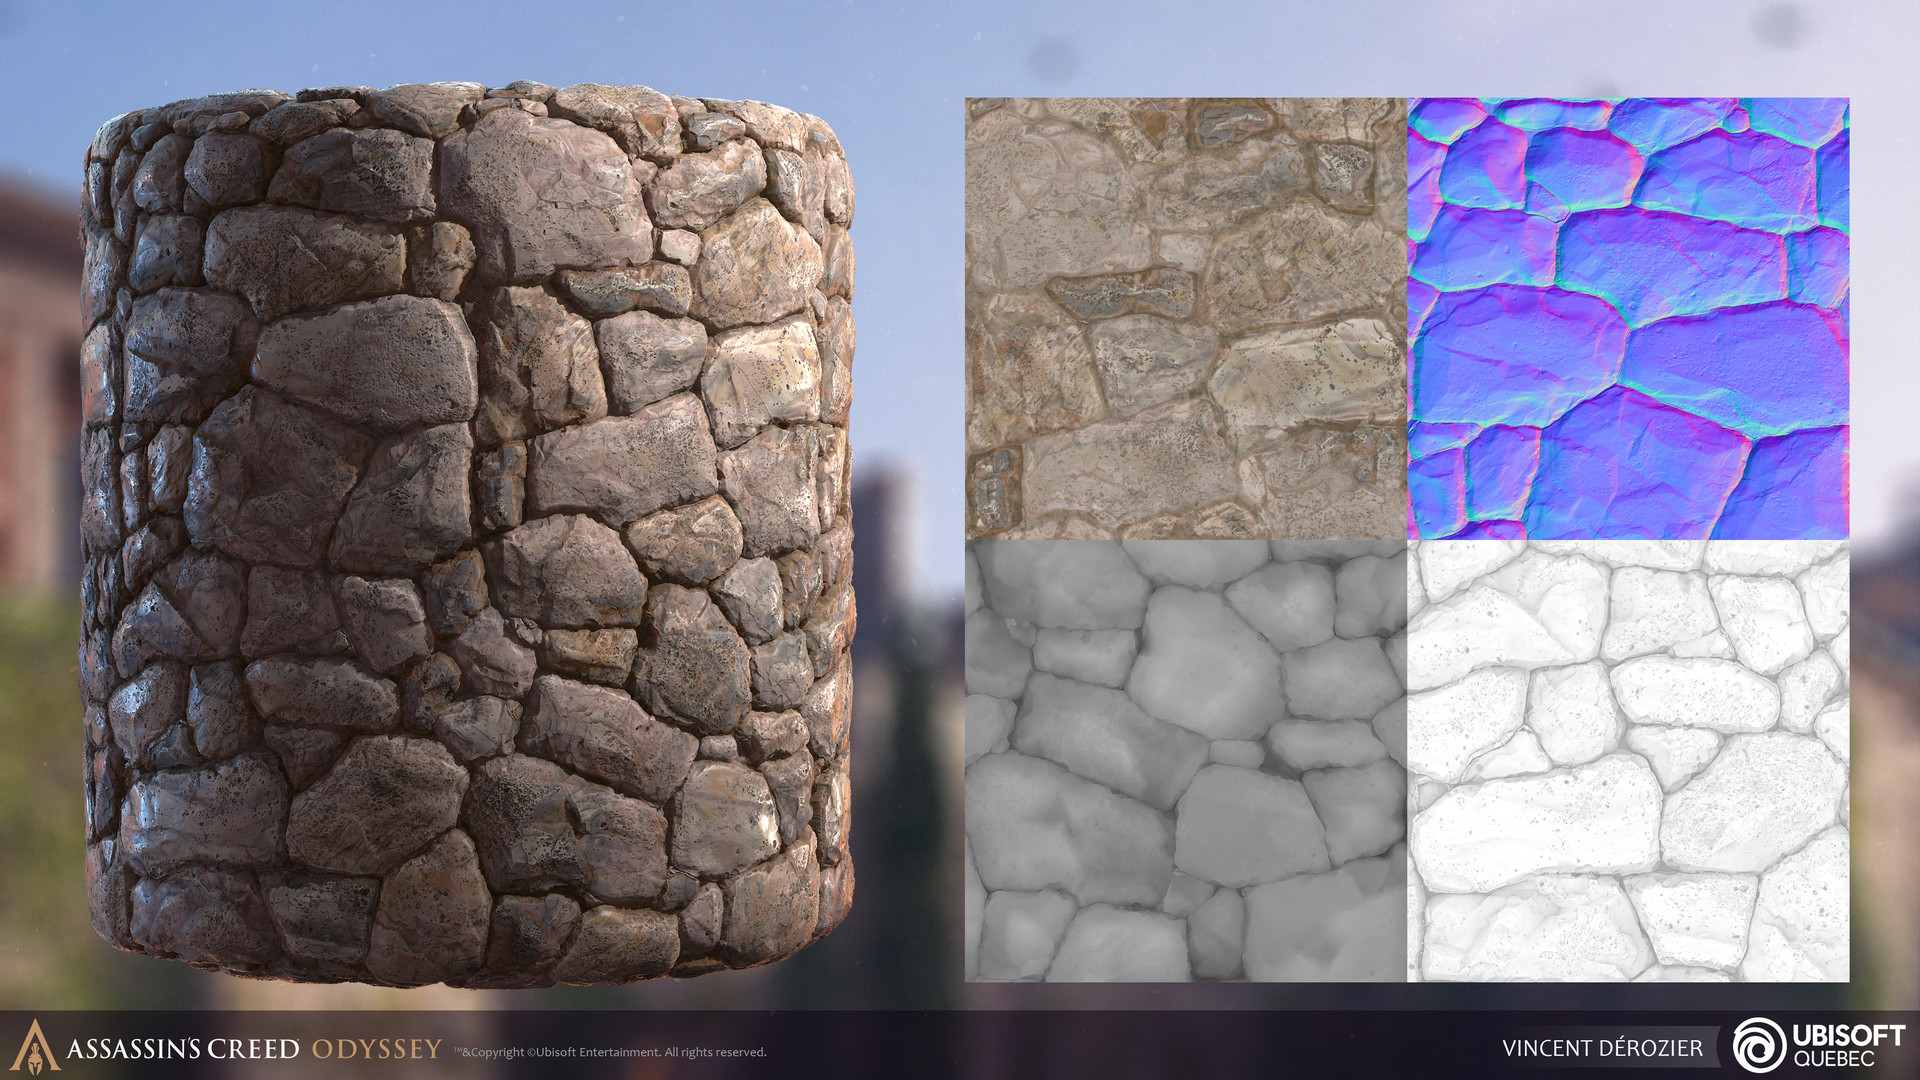
\includegraphics[scale=0.15]{figures/vincent-derozier-assassin-s-creed-odyssey.jpg}
		\caption{PBR render and its maps}
	\end{figure}
\end{frame}

\section{The purpose of parallel processing}
\begin{frame}{Moore's Law}
	Every two years, the density of transistors in an integrated circuit doubles. That means we can compute the critical path of an algorithm faster.
	\begin{figure}
		
\includegraphics[scale=0.2]{figures/buzz1.jpg}
		\caption{\textit{To infinity and beyond!}}
	\end{figure}
\end{frame}

\begin{frame}{Critical path}
	Sometimes, algorithms process data one by one. When applicable, it is necessary to find the critical path and execute it in parallel. Modern CPUs offer the ability to run some threads at the same time. However, CPUs don't have a lot of cores available. For massive parallel computation we will use GPUs.
	\begin{figure}
		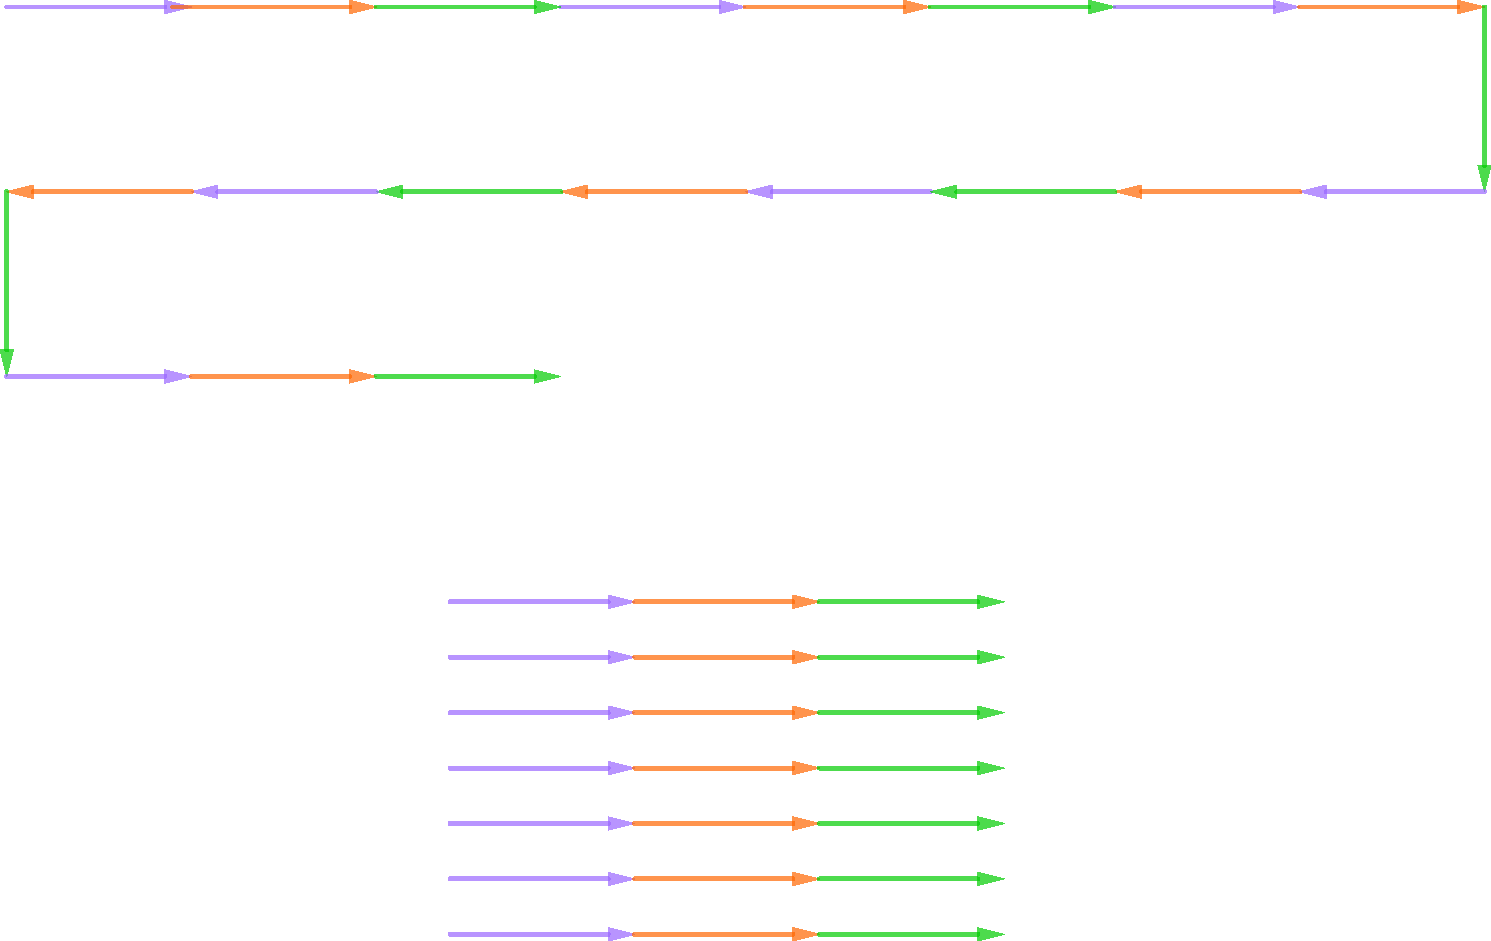
\includegraphics[scale=0.2]{figures/criticalPath.pdf}
	\end{figure}
\end{frame}

\begin{frame}{A world of buffers}
	The aim of parallel computing is solving heavy arithmetic computation on buffer. Single instruction on multiple data. One process is called a kernel for the GPGPU or a shader for the graphics pipeline.
	\begin{figure}
		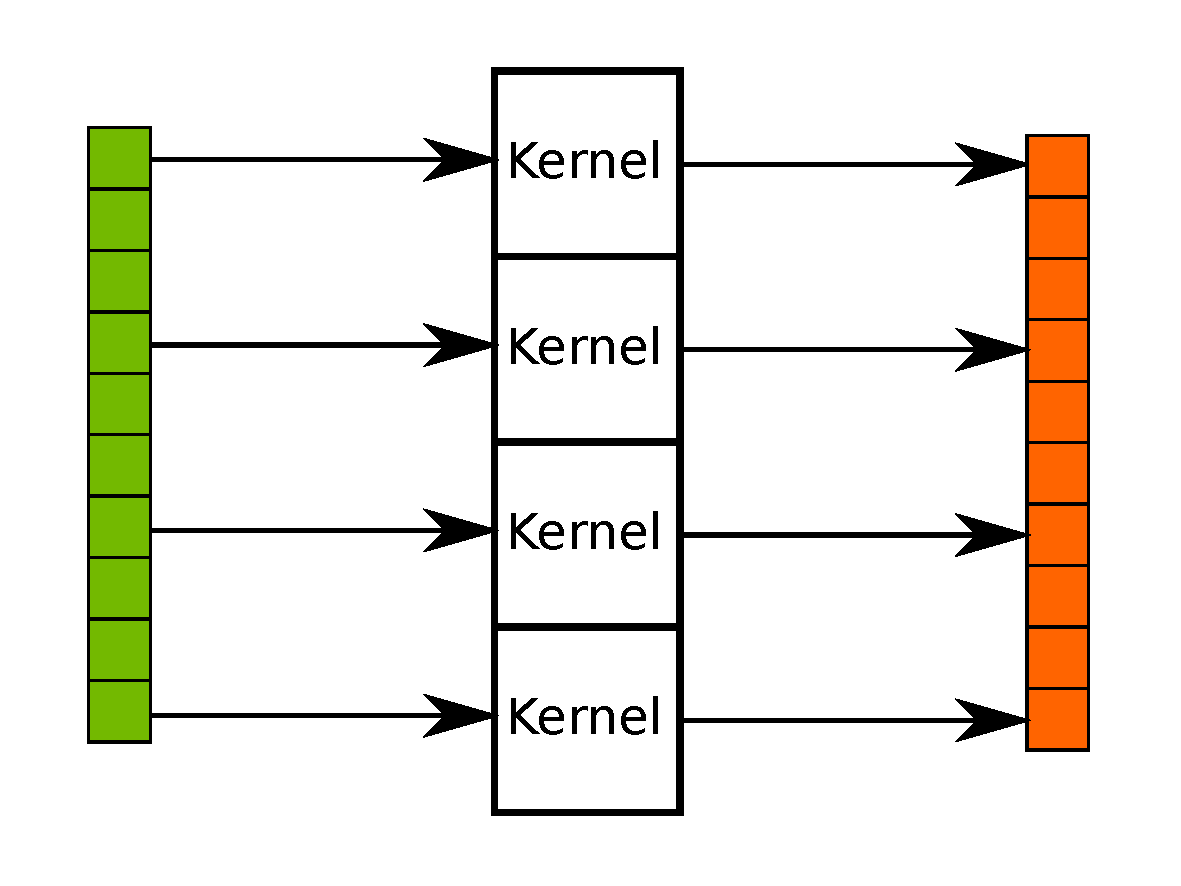
\includegraphics[scale=0.3]{figures/buffer.pdf}
	\end{figure}
\end{frame}

\section{What is a graphic card?}
\begin{frame}{History}
	The first Graphics Processing Unit (GPU) was used for drawing game sprites. It was a dedicated device for formatted data. Ten years after we had the ability to draw lines, fill areas and control the blitter. In 1990, the graphical API appears and allows us to send assembly code to the device.
\end{frame}

\begin{frame}{Arithmetic Logic Unit}
	The Arithmetic Logic Unit (ALU) is the component that performs arithmetic operations. The GPU is more focused on floating point operations, multiple ALUs are combined to create a Floating Point Unit (FPU).
	\begin{figure}
		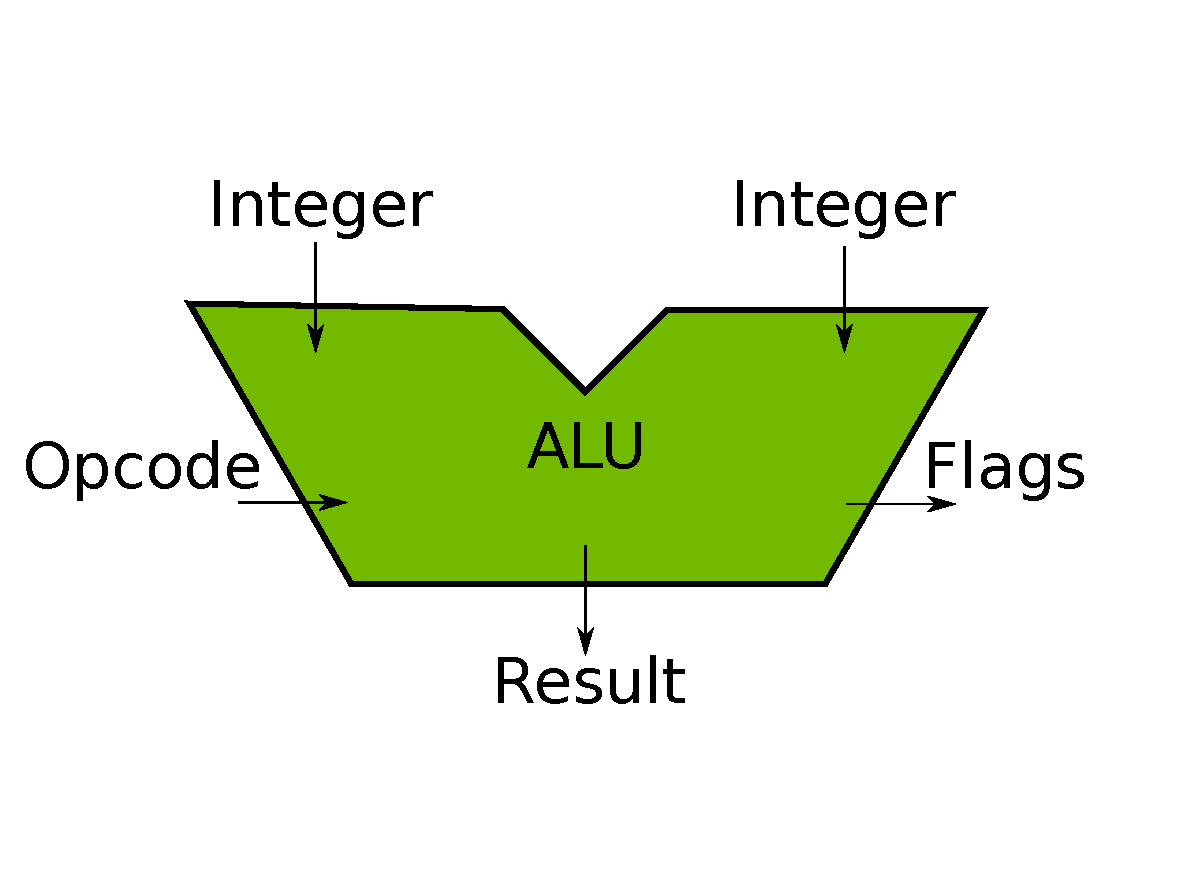
\includegraphics[scale=0.3]{figures/ALU.pdf}
	\end{figure}
\end{frame}

\begin{frame}{CUDA Core}
	CUDA cores are used to execute opcodes from compiled kernels. There are composed of an FPU, logic unit, branch unit and compare unit.
	\begin{figure}
		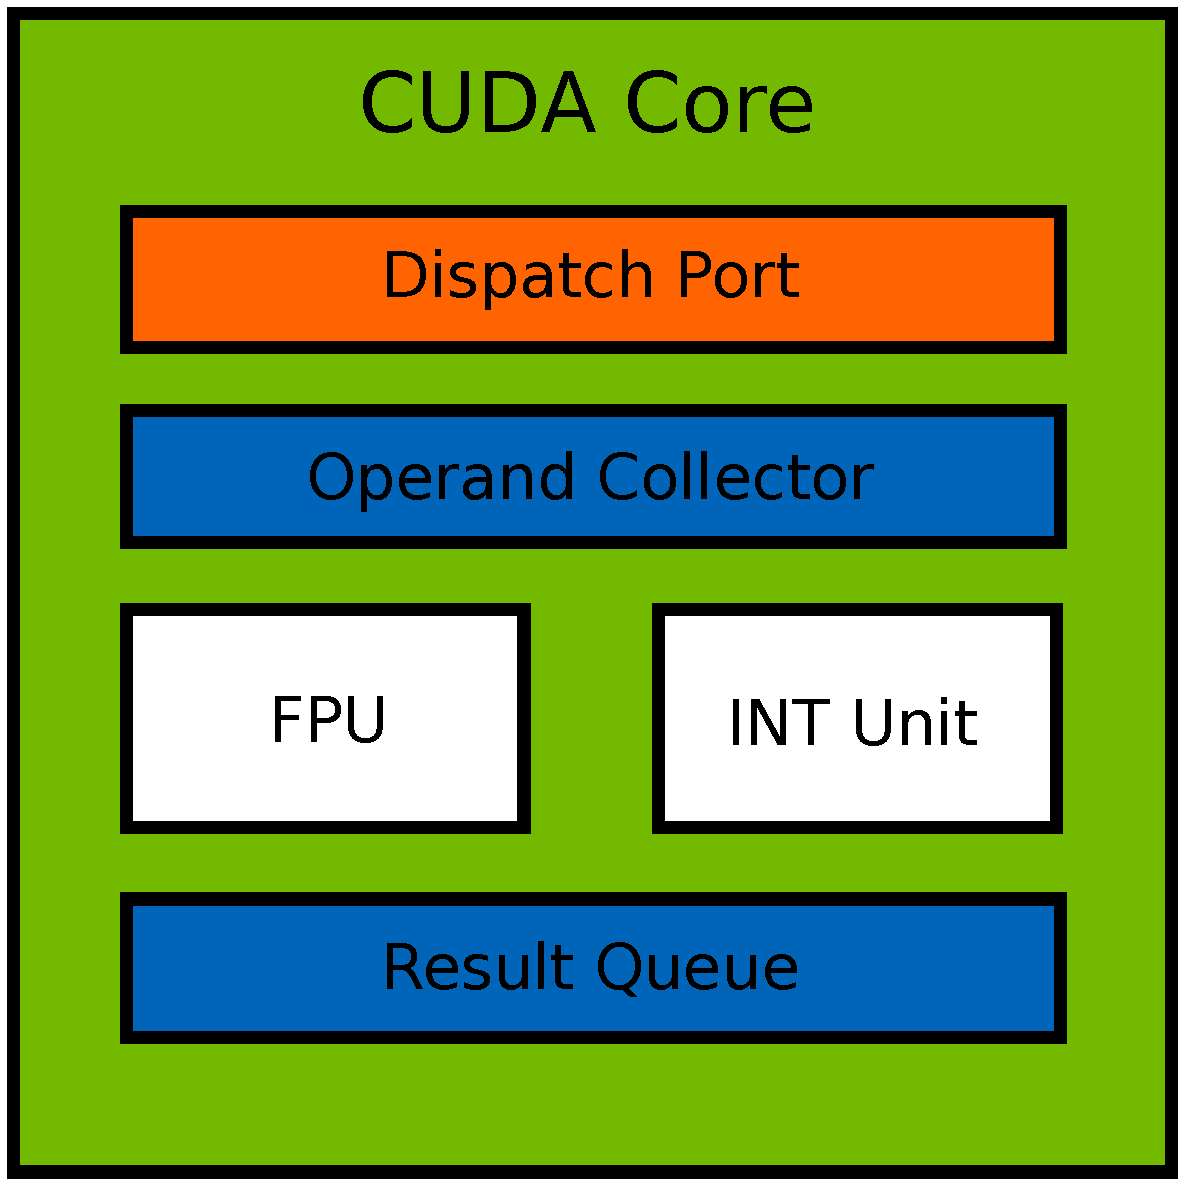
\includegraphics[scale=0.2]{figures/cudacore.pdf}
	\end{figure}
\end{frame}

\begin{frame}{Streaming Multiprocessor}
	The Streaming Multiprocessor (SM) organizes threads in groups of 32 called warp. This architecture is called SPMD (Single Program, Multiple Data).
	\begin{figure}
		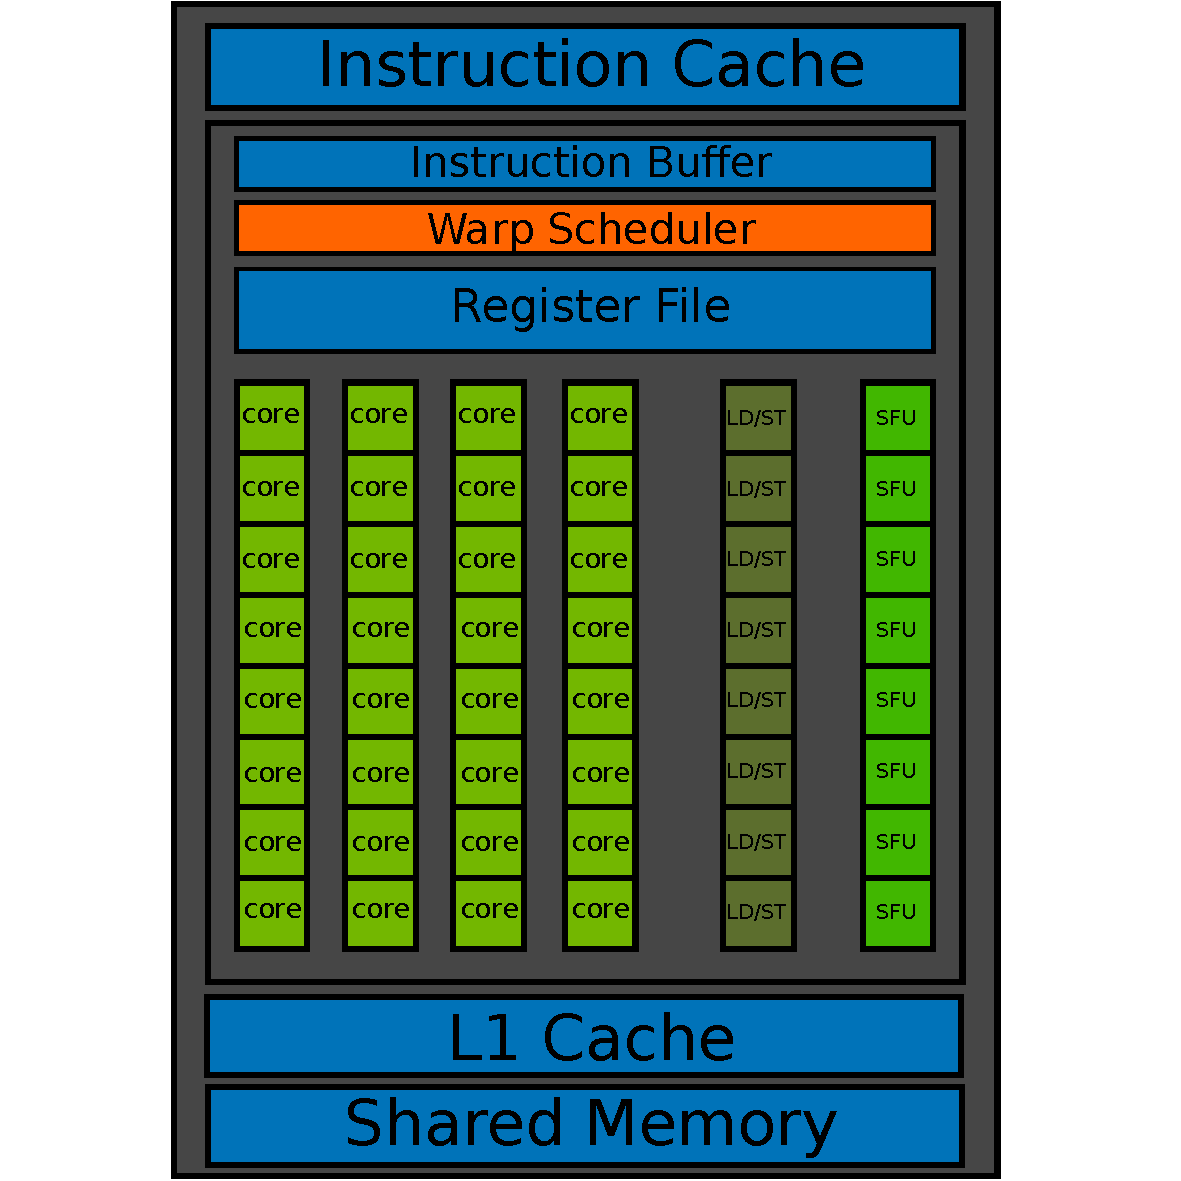
\includegraphics[scale=0.3]{figures/warp.pdf}
	\end{figure}
\end{frame}

\begin{frame}{Streaming Multiprocessor}
	On the GP104 (The GPU of GTX 1080) each SM has four warps. 
	\begin{figure}
		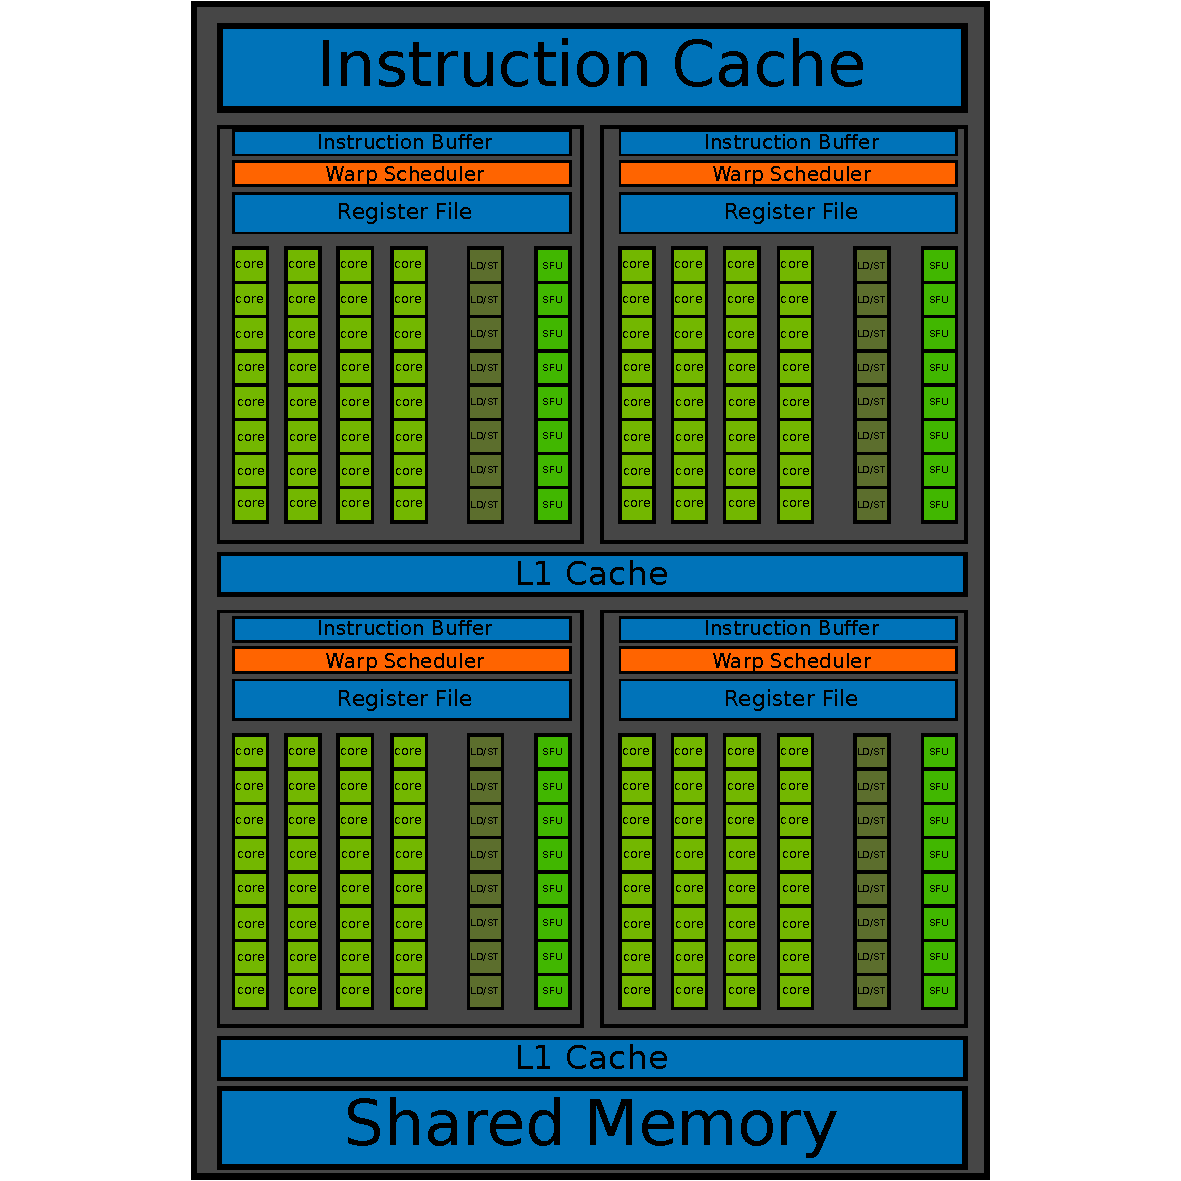
\includegraphics[scale=0.3]{figures/SM.pdf}
	\end{figure}
\end{frame}

\begin{frame}{Graphics Processing Clusters}
	A Graphics Processing Clusters (GPC) is a collection of streaming multiprocessors. In the case of the GP104, there are four clusters.
	\begin{figure}
		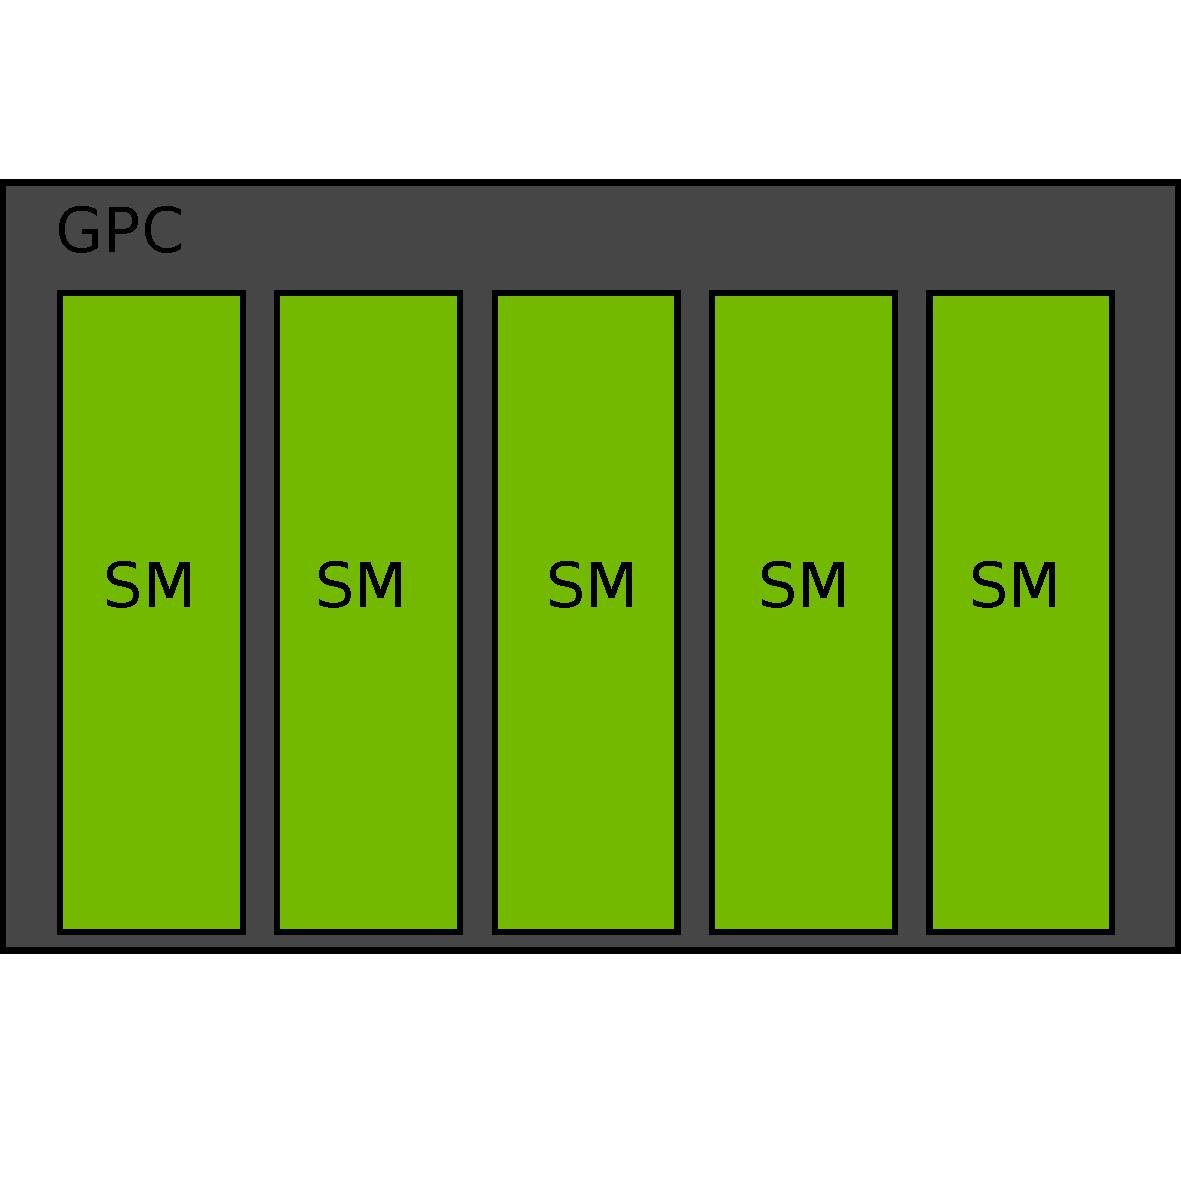
\includegraphics[scale=0.3]{figures/GPC.pdf}
	\end{figure}
\end{frame}

\begin{frame}{GP104}
	All the GPC are connected to the L2 cache memory. The Gigathread engine distributes block threads to streaming multiprocessor. This device has 32 cores * 4 warps * 5 SMs * 4 GPCs = 2560 CUDA cores.
	\begin{figure}
		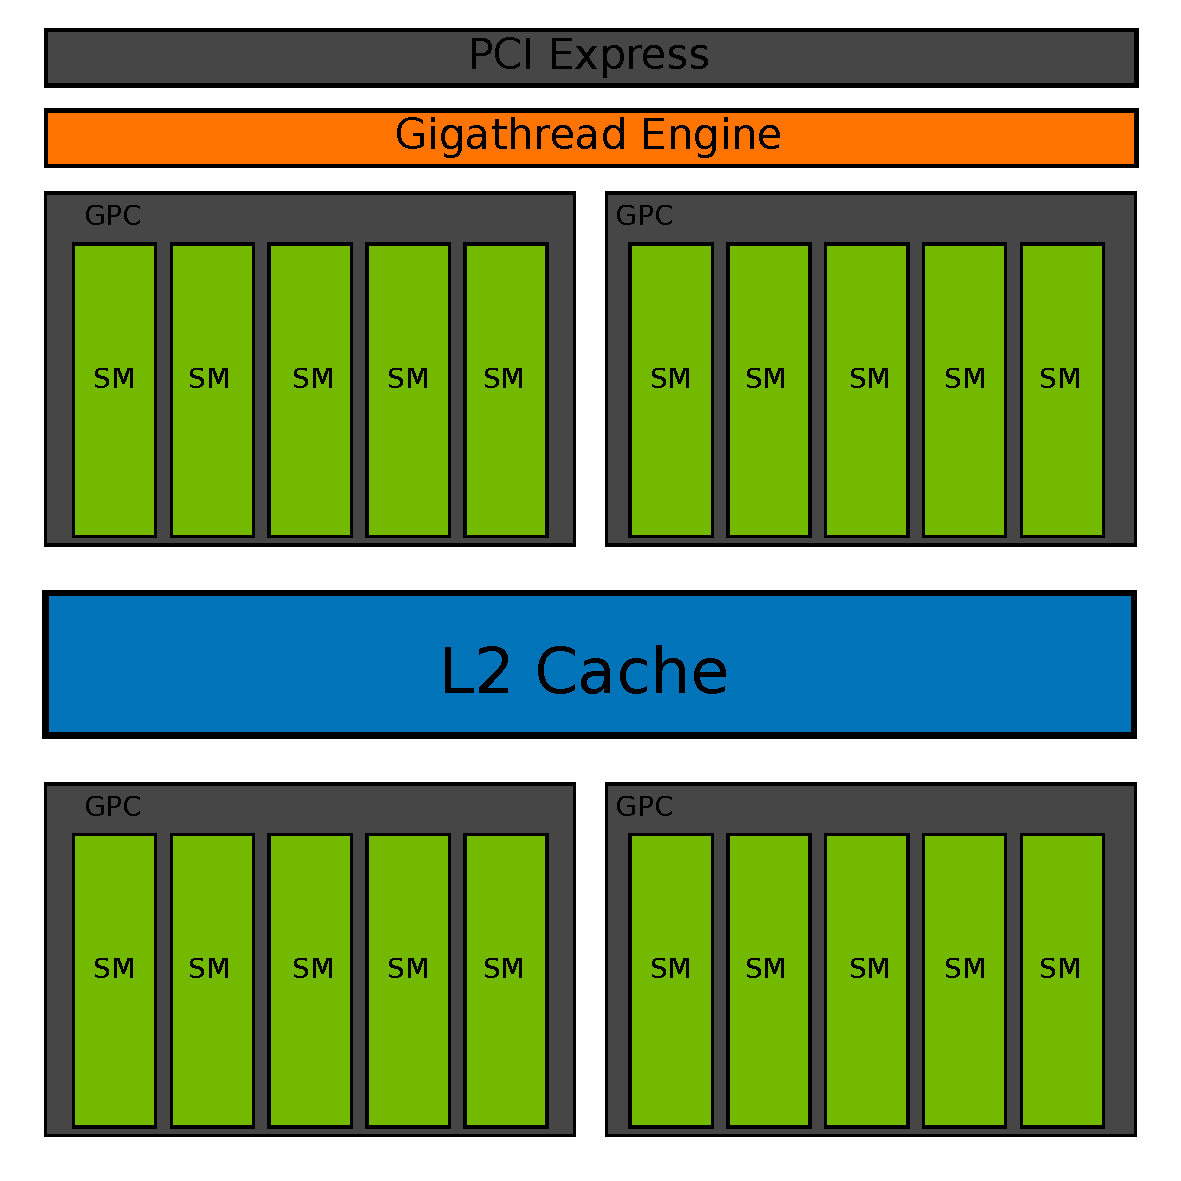
\includegraphics[scale=0.3]{figures/gp104.pdf}
	\end{figure}
\end{frame}

\section{The CUDA language}
\begin{frame}{Host and Devices}
	\begin{itemize}
		\item Host: The CPU and its memory. The host can manage the memory on both the host and the device. The executed code can launch kernels.
		\item Devices: The GPU and its memory. Kernels are executed on many GPU threads in parallel.
	\end{itemize}
\end{frame}

\lstset{language=C++,basicstyle=\ttfamily,keywordstyle=\color{red},commentstyle=\color{green},tabsize=1}

\defverbatim[colored]\codeKernel{
\begin{lstlisting}
	int blocks = 16; // blocks per grid
	int threads = 128; // threads per block
	kernelName<<<blocks, threads>>>();
\end{lstlisting}
}

\begin{frame}{Kernel}
	With CUDA, the kernel declaration is easy. the keyword \_\_global\_\_ has to be added before the kernel function.\\
	The number of threads that execute the kernel is specified by this syntax:
	\codeKernel
\end{frame}

\defverbatim[colored]\codeIndex{
\begin{lstlisting}
	int index = blockIdx * blockDim + threadIdx;
\end{lstlisting}
}

\defverbatim[colored]\codeIndexDim{
\begin{lstlisting}
	int x = blockIdx.x * blockDim.x + threadIdx.x;
	int y = blockIdx.y * blockDim.y + threadIdx.y;
	int z = blockIdx.z * blockDim.z + threadIdx.z;
\end{lstlisting}
}

\begin{frame}{Indexing}
	In the kernel, the threadIdx, the blockIdx and the blockDim allow the user to compute the unique thread id.
	\codeIndex
	If data is stored into 2D or 3D array, it is possible to launch the kernel using a dim3 instead of an integer and the index becomes:
	\codeIndexDim
\end{frame}

\section{GPGPU usage in the industry}
\begin{frame}{APOD}
	The Assess, Parallelize, Optimize, Deploy (APOD) design cycle's goal is to identify and correct bottlenecks into the application. 
	\begin{figure}
		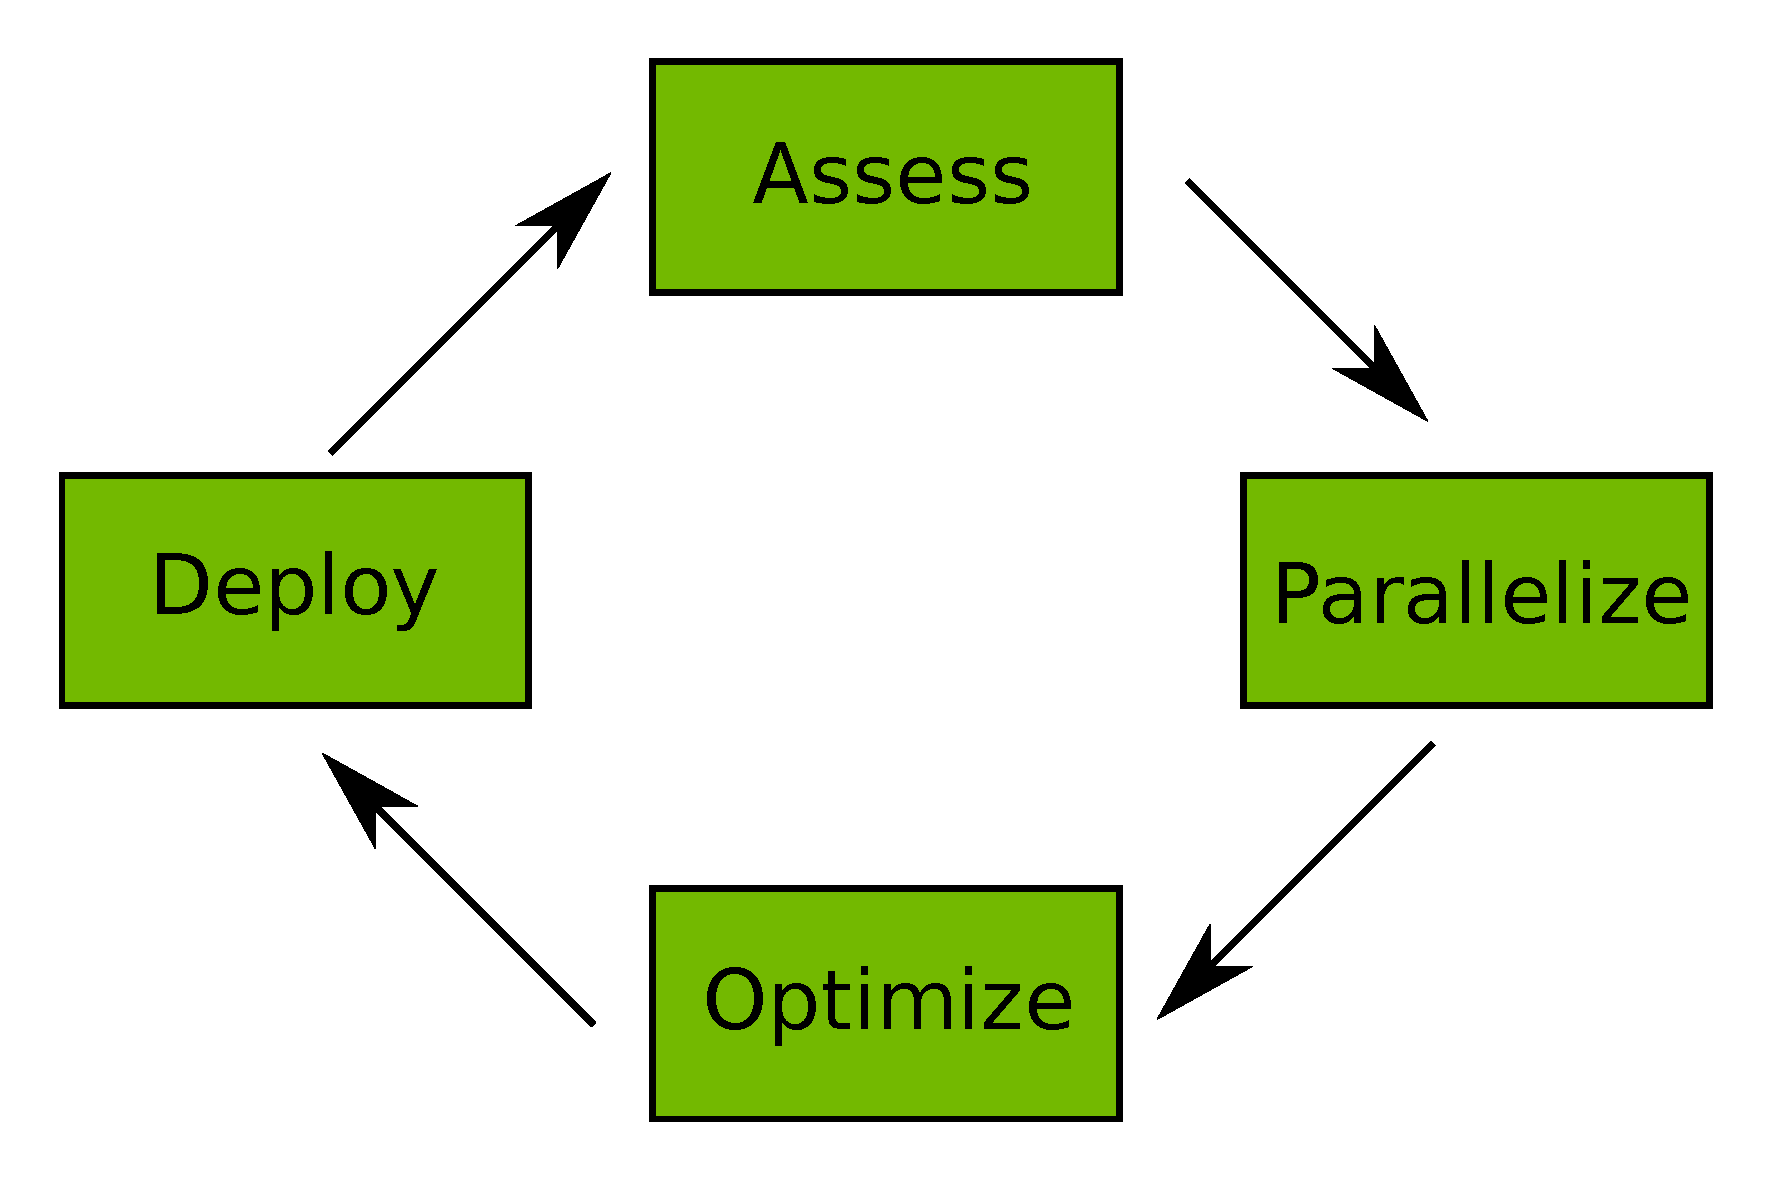
\includegraphics[scale=0.3]{figures/APOD.pdf}
	\end{figure}
\end{frame}

\begin{frame}{Domain Specific}
	\begin{itemize}
		\item Deep Learning
		\item Linear Algebra and Math: Solver, Random function, Finite element method, etc...
		\item Signal
		\item Image and video
		\item Data structure
	\end{itemize}
\end{frame}

\section{Q\&A}

\end{document}
